%%%%%%%%%%%%%%%%%%%%%%%%%%%%%%%%%%%%%%%%%%%%%%%%%%%%%%%%%%%%%%%%%
%                                                               %
%                       Legal Notice                            %
%                                                               %
% This document is copyright (C) Jason Gobat & Darren Atkinson	%
%                                                               %
%%%%%%%%%%%%%%%%%%%%%%%%%%%%%%%%%%%%%%%%%%%%%%%%%%%%%%%%%%%%%%%%%

\newpage{\pagestyle{empty}\cleardoublepage}

\chapter{Structure of a \felt{} Problem}
\label{problem}

\section{Input file syntax}
\label{problem.syntax}
%%%%%%%%%%%%%%%%%%%%%%%%%%%%%%%%%%%%%%%%%%%%%%%%%%%%%%%%%%%%%%%%%%%%%%%%%%%%
A \felt{} problem is defined by an input file which you must create using 
a text-editor such as {\em vi} or from within {\em velvet}
(though in this case you do not actually need to see the resulting 
file).  The input file contains a complete description of everything that 
defines a problem: the nodes, the elements, analysis parameters, 
the constraints and forces on the 
nodes, and the distributed loads and material properties of the elements.  An 
informal description of the file format and these objects is given below.  
For a complete, formal definition of the syntax, you should refer to the 
{\em felt}(4fe) manual page.

\subsection{General rules}

The input file for a typical \felt{} problem will consist of nine sections.
In general, 
each object within a problem ({\tt node, element, force, material, distributed 
load, constraint}) has a symbolic name.  For nodes and elements these names 
are positive integers; for everything else the name is a user assigned string, 
e.g., ``steel'', ``point\_load'', ``roller''.  Each type of object is defined 
within its own section, each section containing a list of definitions for 
objects of that type.  

As a rule of thumb white space can occur anywhere and the 
definition sections can be given in any order (and repeated even).  
The exceptions to this 
are the {\tt problem description} section and the {\tt end}
statement, which must come first and last in an input file, respectively, 
and cannot be repeated. 

Comments are denoted 
as in the C programming language; anything between {\tt /*} and {\tt */}
will be ignored as a comment no matter where it appears in the file. 

\subsection{Expressions}

\subsubsection{Continuous functions}
As a convenience, wherever a numeric value is required for a 
material characteristic, magnitude of a force, load or displacement
boundary condition, or a nodal coordinate, you 
can specify an arbitrary mathematical expression, including the operators
{\tt +, -, *, /, \%} and the 
standard mathematical library functions $sin$, $cos$, $tan$, {\em sqrt},
{\em hypot}, {\em pow}, {\em exp}, {\em log}, {\em log10},
{\em floor}, {\em ceil}, {\em fabs} and {\em fmod}.  Note that arguments
to the trigonometric functions should be given in terms of radians just as
if you were calling them from a C program using the standard math library.
Other than this difference, these functions should be used
and should behave as they are described in the manual pages for your
local mathematics library.

In a transient analysis problem the symbol {\tt t} denotes the time
variable in expressions for force magnitudes or time-varying boundary
conditions.  These expressions will
be dynamically evaulated throughout the course of the simulation.  For other
parameters (loads, nodal coordinates, etc.) and for all parameters in a static
problems, these expressions will simply be evaluated as if {\tt t=0}.
For spectral inputs, the symbol {\tt w} can be substituted for the 
independent variable for clarity and to distinguish frequency domain force
spectra from time domain forces.

Expressions can also
contain the ternary conditional operator as in the C programming language:
``if a then b else c'' is symbolized in a \felt{} input file as 
\mbox{{\tt a ? b : c}} where {\tt a}, {\tt b}, and {\tt c} are all 
valid expressions.  The logical operators to use in constructing {\tt a} are 
the same as those in C ({\tt ==, \&\&, ||, <=, <, >, >=, !=}).  
The conditional construct is particularly useful in defining things like
discontinuous dynamic forces.  

\subsubsection{Discrete functions}
Because some forcing functions are easier to express in a discretized (as 
opposed to continuous) form (e.g., earthquake records), the \felt{} syntax
also includes a mechanism for specifying a discrete representation of a 
transient forcing function.  The basic specification consists of a series of 
time magnitude pairs of the form {\tt (t, F)} where {\tt F} is the value of the
function at time {\tt t}.  In evaluating the function, \felt{} will linearly
interpolate between each adjacent pair for times that fall between two pairs.
A single time magnitude pair will be interpreted as an impulse response
function at the given time.  Note that the pairs must be given in order of 
increasing time.

You can express a periodic discrete function simply by defining one
period and then entering a {\tt +} symbol at the end of the expression.  
You could represent a simple sawtooth forcing function having a period of 
2 seconds and a maximum magnitude of 1000 with an expression like 
\begin{screen}
 \begin{verbatim}
forces
sawtooth Fx=(0,0.0) (2,1000.0)+
 \end{verbatim}
\end{screen}
Figure~\ref{problem.sawtooth} illustrates different ways
to define some common types of loading functions with either continuous
or discrete representations.

\begin{figure}[htb]
 \begin{center}
  \includegraphics[width=6in]{figures/sawtooth}
 \end{center}
 \caption{Example loading functions}
 \label{problem.sawtooth}
\end{figure}

\subsection{Units}

There are no set units for the dimensional quantities that you specify in
defining a problem for \felt{}.  The important thing is to remain consistent
in the units that you use; numerical results will then be consistent with 
the input dimensions.  Some examples of consistent units would be nodal
coordinates in meters, forces in Newtons, elastic moduli in Pascals 
(${\rm N\ m^{-2}}$); moments of inertia would be in ${\rm m^{-4}}$.  The 
displacement results for a problem like this would be in meters; stresses would be
in Pascals.  Convenient English units are often pounds, inches, and 
psi (pounds per square inch) or kips (kilopounds), inches, and ksi.

The \felt{} application, {\em yardstick}, is intended for simple scaling of
the numerical quantities in a \felt{} input file.  As a special case of
this, unit conversion of files is given special treatment and made particularly
easy.  To convert an input file that was originally specified in kips and
feet to Newtons and meters, the {\em yardstick} command line would simply
look like
\begin{screen}
 \begin{verbatim}
% yardstick -if kips -il feet -of N -ol m foo.flt > foo_si.flt
 \end{verbatim}
\end{screen}
The {\em yardstick} manual page details the list of units that the program
recognizes and all of the available options.

\subsection{A simple example}

An input file for a simple 
cantilever beam problem with an end point-load and considering self-weight 
might look something like this:	

\begin{screen}
 \begin{verbatim}
problem description
title="Cantilever Beam Sample Problem" nodes=2 elements=1 analysis=static

nodes
1 	x=0.0	y=0.0	constraint=fixed
2	x=10.0	y=0.0	constraint=free		force=end_load

beam elements
1 	nodes=[1,2]	material=steel		load=self_weight

material properties
steel	A=10.0	E=30e6	Ix=357		/* properties can also be lowercase */

distributed loads
self_weight	direction=perpendicular		values=(1,2000) (2,2000)

constraints
fixed	Tx=C	Ty=C	Rz=C		/* column alignment is unimportant */
free	Tx=U	Ty=U	Rz=U		/* I could have used tx, ty and rz */

forces
end_load	Fy=-1000

end
 \end{verbatim}
\end{screen}

\section{Sections of a \felt{} input file}

\subsection{Problem description}

The {\tt problem description} section is used to define the problem
title and the number of nodes and elements in the problem.  These numbers will
be used for error checking so the specifications given here must match the 
actual number of nodes and elements given in the definition sections.  Note 
that the definitions for nodes and elements do not have to be given in 
numerical order, as long as nodes 1 ... $m$ and elements 1 ... $n$ (where $m$ 
is the number of nodes and $n$ is the number of elements) all get defined in one 
of the element and node definition sections in the file.  The {\tt analysis=}
statement defines the type of problem that you wish to solve.  Currently
it can either be {\tt static}, {\tt transient}, {\tt static-substitution},
{\tt modal}, {\tt static-thermal}, {\tt transient-thermal}, or {\tt spectral}.  
If you do not specify anything, static analysis will be assumed.  The 
{\tt problem description} section is the only section which you cannot repeat 
within a given input file. 

\subsection{Nodes}

The {\tt nodes} section(s) must define all of the nodes given in the problem.  
Each node must be located with an x, y, and z coordinate using {\tt x=},
{\tt y=}, and {\tt z=} assignments.  Coordinates are 
taken as 0.0 if they are not otherwise defined.  If a coordinate is left 
unspecified for a given node, it takes the value for that coordinate from 
the previous node.  A node must also have a constraint assigned to it by a
{\tt constraint=} statement.  The default 
constraint leaves the node completely free in all six degrees of freedom.  
Like coordinates, if a constraint is left unspecified, the node will be 
assigned the same constraint as the previous node.  Forces (applied point 
loads and moments) on a node are optional and are applied using the
{\tt force=} statement; if a force is not specified there 
will be no force applied to that node.  You can also specify an optional
lumped mass at a given node with a {\tt mass=} statement. 

\subsection{Elements}

An element definition section begins with the keywords {\tt xxxxx elements}
where {\tt xxxxx} is the symbolic name of a type of element.  All elements
under this section heading will be taken to be the given element type.
There could be multiple sections that defined beam elements, but each must
begin with the keywords {\tt beam elements}.  If there were truss elements
in the same problem, they would have to be defined in sections which began
with the keywords {\tt truss elements}.  Currently available types 
are {\tt spring}, {\tt truss}, {\tt beam}, {\tt beam3d}, {\tt timoshenko}, 
{\tt CSTPlaneStrain}, {\tt CSTPlaneStress}, {\tt iso2d\_PlaneStrain}, 
{\tt iso2d\_PlaneStress}, {\tt quad\_PlaneStrain}, {\tt quad\_PlaneStress},
{\tt htk}, {\tt brick}, {\tt rod}, and {\tt ctg}.  A \felt{} problem 
is not limited to one element type; the routines for assembling the global 
stiffness matrix takes care of getting the right parts of the right element 
stiffness matrices into the global matrix.  

Each element must have a list of 
nodes to which it is attached.  The node list is defined with the 
\mbox{{\tt nodes=[ \ldots ]}} statement. The length of the list inside the
square brackets varies with element 
type, but must always contain the full number of nodes which the element type 
definition requires (see chapter~\ref{elements} for a complete definition of 
what each type requires).  A material property must also be assigned to every 
element with a {\tt material=} statement.  If the material is never specified, 
an element will take the same material property as the previous element. 
If nothing ever gets assigned to an element, the default material property will 
have zeros for all of its 
characteristics.  Chances are this is not what you want.  Finally, an
element can have up to three optional distributed loads. Each load is assigned
with a separate {\tt load=} assignment.  Each element type may 
treat a distributed load differently so you should be careful that the name 
given for the loads on a given element match the names of distributed loads 
which are defined in a manner conformant with what that element type is 
expecting.	

\subsection{Material properties}

The {\tt material properties}  section(s) is quite simple.  Each material has a 
name followed by a list of characteristics.  Currently available 
characteristics are listed in table~\ref{materials_table}.
\begin{table}
\begin{center}
\small{
 \begin{tabular}{|c|c|}
  \hline
  property name		& description	\\
  \hline\hline
\tt E 		& Young's modulus or elastic modulus \\
\tt A 		& cross-sectional area  \\
\tt t 		& thickness \\
\tt rho 	& density \\
\tt nu 		& Poisson's ratio \\
\tt G 		& bulk or shear modulus \\
\tt J 		& torsional stiffness \\
\tt Ix		& $I_{xx}$ moment of inertia \\
\tt Iy 		& $I_{yy}$ moment of inertia \\
\tt Iz		& $I_{zz}$ moment of inertia \\
\tt kappa 	& shear force correction factor \\
\tt Rk 		& Rayleigh stiffness damping coefficient \\
\tt Rm 		& Rayleigh mass damping coefficient \\
\tt Kx 		& thermal conductivity along the x-direction \\
\tt Ky 		& thermal conductivity along the y direction \\
\tt Kz 		& thermal conductivity along the y direction \\
\tt c 		& heat capacitance  \\
  \hline
 \end{tabular}
}
\end{center}
\caption{Symbolic names used to define material properties}
\label{materials_table}
\end{table}

Note that no element types require a material 
property with every one of these characteristics defined.  In fact, most 
only use three or four characteristics.  You should consult the element 
definitions (chapter~\ref{elements}) for a complete list of what 
each element type requires from a material property.  Density ({\tt rho}) 
is always necessary for the materials in a 
transient, modal, or spectral analysis problem if you actually want your 
elements to have any inertia. Different element types can certainly use the 
same material as long as that material definition contains the right 
characteristics for each type of element that uses it.	

\subsection{Constraints}

The {\tt constraints} section(s) must define all of the named constraints 
within the problem.  Each constraint is defined by a name followed by a list 
of DOF specifications of the form {\tt Tx=? Ty=? Tz=? Rx=? Ry=? Rz=?} 
where the {\tt ?}  
can either be {\tt c} for constrained, {\tt u} for unconstrained or a 
valid, possibly time-dependent, expression for cases where a displacement 
boundary condition is required (e.g., settlement of support, or time-varying
temperature along a boundary in a transient thermal analysis problem).  Note 
that specifiying {\tt Tx=c} is equivalent to {\tt Tx=0.0}.  The {\tt T} and 
{\tt R} refer to 
translation and rotation, respectively and the subscripted axis letter 
indicates that the specification refers to translation along, or rotation 
about, that axis.  An additional specification of {\tt h} or {\tt hinged}
is allowed for the rotational DOFs for cases where it is necessary to model
a nodal (momentless) hinge.  Note that a hinge specification currently
has meaning only on {\tt beam}, {\tt beam3d} and {\tt timoshenko} elements.  

If a specification is never made for a DOF, then
the problem is assumed to be unconstrained in that degree of freedom.
Getting the constraints right is an important part 
of getting a reasonable solution out of a finite element problem so you
should be aware of what DOF are active in a given problem (this will 
depend on which types of elements are being used ... even in a 2-d problem, 
the global stiffness matrix will take displacement in the z direction into 
account if there are 3-d elements in use, consequently, those displacements 
should be constrained).	

In order to account for initial conditions in transient analysis
problems, a constraint specification may also include the initial (at time
$t=0$) displacements, and velocity
and acceleration in the translational DOFs.  Initial displacements are given
with {\tt ITx=}, {\tt IRz=}, etc.  You can specify initial accelerations with
{\tt Ax=}, {\tt Ay=}, and {\tt Az=}. Initial velocities are given by {\tt Vx=},
{\tt Vy=}, and {\tt Vz=}.  Unspecified velocities and displacements will be 
taken as 0.0.  If there are no initial accelerations specified (i.e., none of 
the nodes have a constraint with an acceleration assigned) then the initial 
acceleration vector will be solved for by the mathematical routines based on 
the initial force and velocity vectors.  If any of the
nodes have a constraint which has an acceleration component defined (even
if that component is assigned to 0.0) then the mathematical routines will
not solve for an initial acceleration vector; they will build one based
on the constraint information, assigning 0.0 to any component that was
not specified.  What this means is that you cannot specify the initial
acceleration for only a few nodes and expect the mathematical routines
to simply solve for the rest of them. If you specify any of the initial
accelerations then you are effectively specifying all of them.

\subsection{Forces}

The {\tt forces} section(s) defines all of the point loads used in the problem 
and actually looks a lot like the {\tt constraints} section.  The magnitudes of 
the forces in the six directions are specified by {\tt Fx=? Fy=? Fz=? Mx=? 
My=? Mz=?}.  If the value for a given force component is not given it is 
assumed to be zero.  The directions for both forces and the constraints as 
defined above should be given in the global coordinate system (right-hand 
Cartesian). 

If you are doing transient analysis, the force definitions can be more
complicated than a simple numerical assignment or expression.  \felt{}
allows you to specify a transient force as either a series of time-magnitude 
pairs (a discrete function in time) or as an actual continuous function of 
time.  This latter fact means that you can define a force as {\tt Fx=sin(t)}
rather than having to discretize the sine function.  These continuous
forcing functions are a special case of expressions as discussed above.

For spectral analysis problems, you can explicitly specify input
spectra using {\tt Sfx=}, {\tt Smy=}, etc. if you want to to compute the
actual power spectrum of the output.  These spectra can be analytic
functions of {\tt w} or discrete frequency, power pairs.

\subsection{Distributed loads}

The {\tt distributed loads} section(s) must contain a definition for
each distributed load that was assigned in the element definition
section(s).  A valid definition for a distributed load is a symbolic
name followed by the keywords {\tt direction=xxx} and 
{\tt values=(n,x) (m,y) \dots}.  The direction assignment must be set to one of 
{\tt parallel, perpendicular, LocalX, LocalY, LocalZ, GlobalX, GlobalY, 
GlobalZ, radial, axial}. 
The valid directions for a given element type, and what those
directions refer to for that element type are described in the individual
element descriptions in chapter~\ref{elements}.  The values assignment is used 
to assign a list of load pairs to the named load.  A load pair is given in the 
form {\tt (n, x)} where {\tt n} is the local node number to which the magnitude 
given by {\tt x} applies.  Generally, two pairs will be required after the
{\tt values=} token.  The imaginary line between the two magnitudes at
the two nodes defines an arbitrarily sloping linearly distributed load.
This allows you to specify many common load shapes: a constant
distributed load of magnitude $y$, including cases of self-weight, a
load which slopes from zero at one node to $x$ at a second node, or a
linear superposition of these two cases in which the load has magnitude
$y$ at node 1 and magnitude $x+y$ at node 2.  This latter case is
illustrated in figure~\ref{problem.load_fig}.  The definition of this
load would be 

\begin{screen} 
 \begin{verbatim} 
distributed loads
load_case_1    direction=perpendicular    values=(1,-2000) (2,-6000)
 \end{verbatim} 
\end{screen}

In the future, higher-order load shapes may be 
supported by some elements and thus require the specification of more than 
two load pairs.	

\begin{figure}
 \begin{center}
  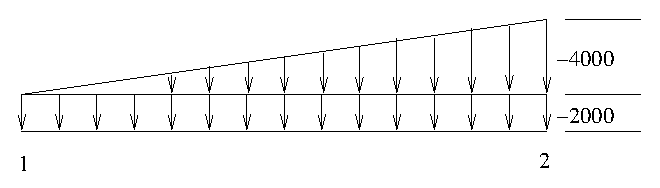
\includegraphics[width=5in]{figures/load_fig}
 \end{center}
 \caption{An example of a complex distributed load.}
 \label{problem.load_fig}
\end{figure}

\subsection{Analysis parameters}

The {\tt analysis parameters} section is required only if you are doing
some type of transient, modal, or spectral  analysis (e.g., 
{\tt analyis=transient}, {\tt analysis=spectral}
in the {\tt problem description} section).  For modal analysis it is simply
used to set the type of element mass matrices that will be formed, but for 
transient and spectral analyses it contains information that further defines 
the problem and the parameters for the numerical integration in time. The 
variables that you can define in this section include: {\tt start=} for
the start of the frequency range of interest in spectral analyis;
{\tt stop=} for the end of the time (transient analysis) or frequency
(spectral analysis) range of interest ({\tt duration=} is an alias for
{\tt stop=}); {\tt step=} for the time or frequency step to be used between
the start and stop points ({\tt dt=} is an alias for {\tt step=});
{\tt beta=}, {\tt gamma=}, and {\tt alpha=} for integration 
parameters in the structural and thermal dynamic integration schemes;
{\tt mass-mode=} for 
the types of element mass matrices that should be formed, either {\tt lumped}
or {\tt consistent} (note again that this is the only assignment that is 
required in this section for a modal analysis problem); {\tt nodes=[ ... ]} 
defines a list of nodes which you
are interested in seeing output for; {\tt dofs=[ ... ]} defines the list
of local DOF that you are interested in for the nodes that you are interested in.
The list of nodes should just be a comma delimited list of node numbers.
The list of DOF should be a list of symbolic DOF names ({\tt Tx, Ty, Tz, Rx,
Ry, Rz}).  You will get solution output for each of these DOF at each of the
nodes that you specified in the node list.  Finally, you can specify 
global Rayleigh damping parameters with {\tt Rk=} and {\tt Rm=}.  If either
of these parameters is non-zero then the global damping matrix will be
formed using these two parameters and the global mass and stiffness matrices
as opposed to being formed from elemental Rayleigh parameters and elemental
mass and stiffness matrices.

You should refer to the chapter
on algorithmic details (section~\ref{algorithms.analysis}) for a little more 
insight on the meanings of the
integration parameters.  The individual element descriptions in 
chapter~\ref{elements} discuss the different mass matrices for that element.
The analysis parameters and their meaning are summarized in 
table~\ref{analysis_table}.
\begin{table}
 \begin{center}
\small{
  \begin{tabular}{|c|l|l|c|c|}
\hline
parameter & description	& example & r/o \\
\hline\hline
start     & frequency range start (SP), load range start (LR) & 0.0 & r \\
stop      & time- (T, TT), frequency- (SP) or load- (LR) range end & 10.0 & r \\
step      & time- (T, TT), frequency- (SP) or load- (LR) step & 0.05 & r \\
alpha	  & $\alpha$ in HHT-$\alpha$ and transient thermal integration (T, TT) & 0.5 & o \\
gamma	  & $\gamma$ in HHT-$\alpha$ integration (T) & 0.25 & o \\
beta	  & $\beta$ in HHT-$\alpha$ integration (T) & 0.5 & o \\
mass-mode & element mass matrices to use (T, TT, SP, M) & {\tt lumped} & r \\
nodes     & list of nodes for which you want results (T, TT, SP, LR, LC) & [1,4,5] & r \\
dofs	  & list of DOF at each result node (T, TT, SP, LR, LC) & [Tx, Rz] & r \\
Rk	  & global Rayleigh damping constant for stiffness (T, M, SP) & 3.0 & o \\
Rm	  & global Rayleigh damping constant for mass (T, M, SP) & 1.4 & o \\
input-node & node to be parametrically excited (LR)         & 4     & r \\
input-dof  & DOF at the input node to be excited (LR)       & Ty    & r \\
tolerance  & convergence tolerance (SUB)	              & 1e-3  & r \\
iterations & maximum permitted number of iterations (SUB)   & 100   & r \\
relaxation & under- (over-) relaxation factor (SUB)         & 0.8   & r \\
load-steps & number of incremental steps to full load (SUB) & 10    & r \\
\hline
   \end{tabular}
}
  \end{center}
\caption[Meaning given to the various analysis parameters.]
        {Meaning given to the various analysis parameters.  T indicates 
         transient analysis; TT is transient-thermal; SP is spectral; 
         M is modal; LR is static analysis (linear or nonlinear) 
         with load ranges; LC is 
         static analysis (linear or nonlinear) with load cases; 
         SUB is non-linear static
         substitution analysis.  The r/o column indicates whether the 
         parameter is (r)equired for the given analyses or if the 
         (o)ptional default value of 0.0 will be used if nothing is specified.}
\label{analysis_table}
\end{table}

\subsection{Load cases}


\section{An illustrated example}
\label{problem.example}

Figure~\ref{problem.example1} illustrates a slightly more complicated 
problem,  a 
simply supported beam with two triangular loads applied and a spring support 
at the center.  We can model the spring as a slender truss element such that
$EA/L = k$, the spring stiffness.  

\begin{figure}[htb]
 \begin{center}
  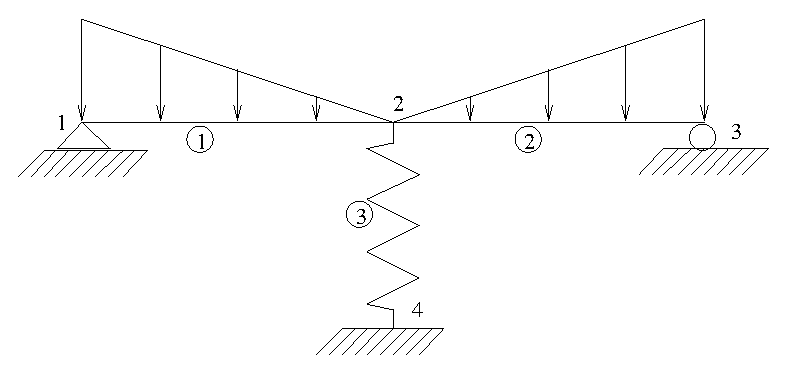
\includegraphics[width=5.5in]{figures/example1}
 \end{center}
 \caption{A mixed element problem with distributed loads.}
 \label{problem.example1}
\end{figure}

The input file for this problem would probably look something like this.
\begin{screen}
 \begin{verbatim}
problem description
title="Mixed Element Sample" nodes=4 elements=3

nodes
1     x=0     y=0     constraint=pin
2     x=6     y=0     constraint=free
3     x=12    y=0     constraint=roller
4     x=6     y=-10   constraint=fixed

beam elements
1 nodes=[1,2]     material=steel     load=left_side
2 nodes=[2,3]                        load=right_side

truss elements
3 nodes=[2,4]     material=spring

material properties
steel    A=1          E=210e9     Ix=4e-4
spring   A=4.76e-7    E=210e9			/* k = 10 kN/m */

constraints
pin     Tx=c Ty=c Tz=c Rz=u	/* we better constrain Tz because */
free    Tx=u Ty=u Tz=c Rz=u	/* there is a truss element!      */ 
roller  Tx=u Ty=c Tz=c Rz=u  
fixed   Tx=c Ty=c Tz=c Rz=c  

distributed loads
left_side      direction=perpendicular   values=(1,10000) (2,0)
right_side       direction=perpendicular   values=(1,0) (2,10000)

end
 \end{verbatim}
\end{screen}

\section{An example of a transient analysis problem}
\label{problem.transient}

Figure~\ref{problem.example2} illustrates a simple frame problem subjected
to a time-dependent loading.  Our input file for this problem differs
from our above example in only one significant way;
we must include an {\tt analysis parameters} section in this case.
Also we need to remember to define the density of all the materials
so we can get a proper mass matrix for each element.  In this case
we have also calculated what the self-weight effect of this mass will
be assuming bays on 15 ft centers (depth of frame into page) and assigned 
it to each element as a distributed load in terms of pounds per inch.

\begin{figure}[htb]
 \begin{center}
  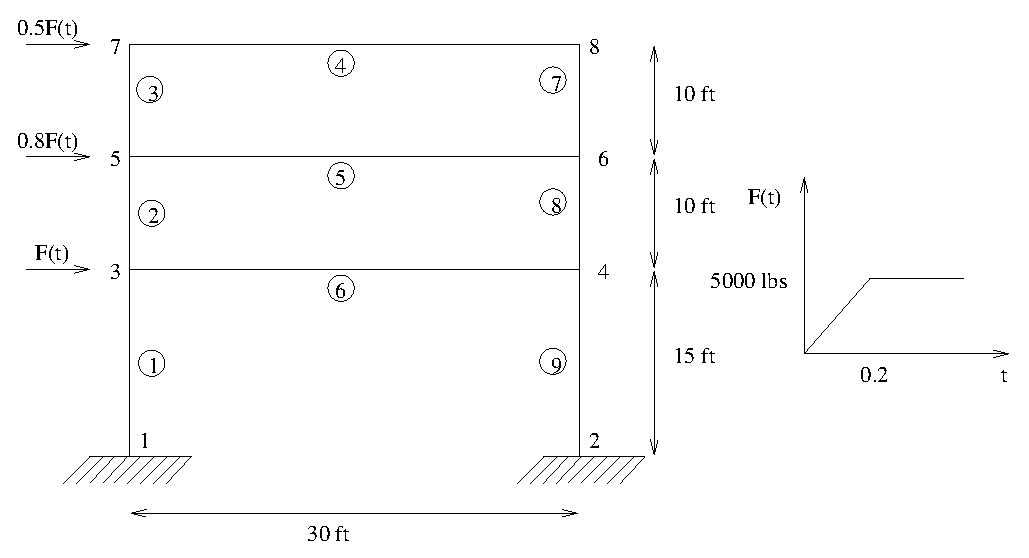
\includegraphics[width=6in]{figures/example2}
 \end{center}
 \caption{Transient analysis of a simple frame structure.}
 \label{problem.example2}
\end{figure}

The input file for this case could look something like the following.

\begin{screen}
 \begin{verbatim}
problem description
title="Dynamic Frame Analysis" nodes=8 elements=9 analysis=transient

analysis parameters
dt=0.05    duration=0.8
beta=0.25  gamma=0.5  alpha=0.0
nodes=[8]  dofs=[Tx]  mass-mode=lumped

nodes
1 x=0   y=0   constraint=fixed
2 x=360 y=0
3 x=0   y=180 constraint=free   force=f1
4 x=360     
5 x=0   y=300                   force=f2
6 x=360
7 x=0   y=420                   force=f3
8 x=360

beam elements
1 nodes=[1,3] material=wall_bottom
2 nodes=[3,5] material=wall_top
3 nodes=[5,7] 
4 nodes=[7,8] material=floor_top      load=top_wt    
5 nodes=[5,6] material=floor_bottom   load=bottom_wt
6 nodes=[3,4]                         load=bottom_wt
7 nodes=[8,6] material=wall_top	     
8 nodes=[6,4]
9 nodes=[4,2] material=wall_bottom

material properties
wall_bottom  A=13.2 Ix=249 E=30e6 rho=0.0049    /* rho is in lb-s^2/in^4 */
wall_top     A=6.2  Ix=107 E=30e6 rho=0.0104
floor_top    A=12.3 Ix=133 E=30e6 rho=0.01315
floor_bottom A=24.7 Ix=237 E=30e6 rho=0.0136

distributed loads
top_wt    direction=perpendicular    values=(1,-62.5) (2,-62.5)
bottom_wt direction=perpendicular    values=(1,-130) (2,-130)

forces
f1 Fx=1000*(t < 0.2 ? 25*t : 5)
f2 Fx=800*(t < 0.2 ? 25*t : 5)
f3 Fx=500*(t < 0.2 ? 25*t : 5)

constraints
fixed Tx=c Ty=c Rz=c
free  Tx=u Ty=u Rz=u

end
 \end{verbatim}
\end{screen}

\section{Format conversion}

Any problem that you want to solve with \felt{} must be formatted according
to the rules that we have just described.  However, we recognize that
there are countless other formats that provide for descriptions of these 
same kinds of problems (at least the geometric aspects of the problem). 
Because of this, \felt{} provides a mechanism for translating back and forth
between \felt{} and alternative syntaxes. 

\subsection{Conversion basics}

A common example of a popular geometric description syntax is DXF (drawing 
interchange format).  DXF files can be produced by any number of CAD and
geometric modeling programs.  The \felt{} conversion tool, {\em patchwork},
can translate DXF files to and from the \felt{} syntax.  {\em patchwork}
is invoked with a command-line like:

\begin{screen}
 \begin{verbatim}
% patchwork -dxf bridge.dxf -felt bridge.flt
 \end{verbatim}
\end{screen}

This example would convert the geometric description given in the file
{\tt bridge.dxf} to the geometric basics of a standard \felt{} file,
{\tt bridge.flt}.  Geometric basics in this case means that only the
nodes and elements sections will be translated; the DXF file cannot contain
any information about material properties, forces, loads, constraints, and
therefore this information will be left incomplete in the resulting \felt{}
file.

{\em patchwork} can also translate \felt{} files into other formats.  You
might want to do this if you had used some of \felt{}'s mesh generation 
capabilities for the bulk of your geometric problem description, but wanted
to do some refinement using your favorite CAD program.  The {\em patchwork}
command line to do something like that is simply the reverse of above:
\begin{screen}
 \begin{verbatim}
% patchwork -felt mesh.flt -dxf mesh.dxf 
 \end{verbatim}
\end{screen}

\subsection{{\em patchwork} details}

{\em patchwork} operates by providing routines to read and write the different
file formats based around a single data structure.  The input formatted file
is translated into the uniform database and then the output formatted file
is generated from this same database.  The ability to read or write
any given format is dependent on whether or not routines exist to go
back and forth between the file syntax and the uniform data structure.
Currently, {\em patchwork} can read (i.e., the allowable input formats are)
DXF files, standard \felt{} files, and data files formatted for use in graphing
applications like {\em gnuplot}; {\em patchwork} can write (i.e.,
allowable output formats are) \felt{}, DXF, {\em gnuplot}, and files formatted 
for the software that is distributed with Logan's introductory finite element 
text \cite{logan:fem}.  Capabilities for additional formats will be added
as time permits and demand warrants.  Note that the DXF handling routines 
are limited to line and polygonal polyline entities.

When invoking {\em patchwork}, the input format and file always come
first.  The syntax is \mbox{{\tt patchwork -[iformat] ifile -[oformat] ofile}},
where {\tt [iformat]} can currently be one of {\tt dxf, felt, graph} and
{\tt [oformat]} can be one {\tt dxf, felt, graph, logan}.  An input
or output file name of {\tt -} (a hyphen) indicates that input should be read
from standard input and/or output should be written to standard output,
respectively.
